% Presentación oral del TP4. Mismo formato Beamer que el TP3.
\documentclass[aspectratio=169,11pt]{beamer}
\usetheme{Warsaw}
\useoutertheme{miniframes}
\setbeamertemplate{navigation symbols}{}
\setbeamertemplate{footline}[frame number]
\let\originalpercent\%
\usepackage[spanish,es-noquoting]{babel}
\AtBeginDocument{\let\%\originalpercent}
\usepackage{amsmath,amssymb,graphicx,booktabs,xcolor,tikz}
\usetikzlibrary{positioning,arrows.meta,shapes.multipart}

\definecolor{itbablue}{RGB}{0,91,145}
\definecolor{accent}{RGB}{211,92,32}
\definecolor{softblue}{RGB}{232,243,249}
\definecolor{fresh}{HTML}{1F5FBF}
\definecolor{used}{HTML}{D0392F}
\setbeamercolor{structure}{fg=itbablue}
\setbeamercolor{alerted text}{fg=accent}
\setbeamercolor{block title}{fg=white,bg=itbablue}
\setbeamercolor{block body}{bg=softblue}
\setbeamerfont{frametitle}{size=\large}
\setbeamerfont{title}{size=\LARGE}
\setbeamertemplate{section page}{\vfill\centering{\usebeamercolor[fg]{structure}\usebeamerfont{title}\insertsectionhead\par}\vfill}
\graphicspath{{figuras/}}

\newcommand{\pasoElegido}{2\times10^{-5}}
\newcommand{\rapidezRealizaciones}{30}
\newcommand{\tEstacionario}{1}
\newcommand{\deltaEElegido}{(2{,}6\pm1{,}0)\times10^{-4}}
\newcommand{\cpu}{Intel Core i7-1165G7}
\newcommand{\rendimientoTexto}{\textbf{Al duplicar $N$} ($100\to200\to400$)\\TP4: $\times1{,}8$ y $\times2$\\TP3: $\times9{,}7$ y $\times19$\\TP3 más rápido hasta $N=400$\\$N=650$: TP3 tarda $\times10$}
\newcommand{\kbtAjuste}{(1{,}242\pm0{,}007)\times10^{-2}}
\newcommand{\cineticaMedia}{(1{,}2323\pm0{,}0005)\times10^{-2}}
\newcommand{\posicionTexto}{\textbf{Menor $\langle t_{90}\rangle$}\\$N=100$: $x_0=0{,}16$ m\\\quad $14{,}7\pm1{,}6$ s\\\quad a menos de $1\sigma$: 0{,}16 a 0{,}30 m\\$N=20$: $x_0=0{,}40$ m\\\quad $11\pm3$ s\\\quad a menos de $1\sigma$: 0{,}11 a 0{,}40 m}
\newcommand{\mapaTexto}{Círculo: mínimo de cada $N$\\$N=20$: $11\pm3$ s\\$N=50$: $13\pm2$ s\\$N=100$: $14{,}7\pm1{,}6$ s\\$N=200$: $19{,}8\pm1{,}4$ s\\Todas las realizaciones llegan a $F_{\mathrm u}=0{,}9$}
\newcommand{\densidadTexto}{\textbf{No llegan todas antes de $t_f$}\\$t_{100}$: desde $N=400$ (3 de 10)\\$t_{90}$: desde $N=550$ (3 de 10)\\\textbf{$\fu(t_f)$ sin $t_{90}$}\\$N=550$: $0{,}908\pm0{,}011$\\$N=600$: $0{,}698\pm0{,}011$\\$N=650$: $0{,}046\pm0{,}005$}

\expandafter\newcommand\csname enlacedensidad\endcsname{\url{https://youtu.be/c9ZH7KlfAuU}}
\expandafter\newcommand\csname enlaceposicion\endcsname{\url{https://youtu.be/-nXT0ijHLjg}}
\expandafter\newcommand\csname enlacerapidez\endcsname{\url{https://youtu.be/0tM7ojqST2Y}}


\newcommand{\vect}[1]{\mathbf{#1}}
\newcommand{\fu}{F_{\mathrm u}}
\newcommand{\dt}{\Delta t}
% Grupos de texto sin fondo ni borde, con títulos y espaciado comunes.
\newcommand{\ficha}[3][itbablue]{%
  \par
  \begingroup
    \begin{minipage}{\linewidth}
    {\small\bfseries\color{#1}#2\par}\vspace{3pt}
    {\small\raggedright
      \setlength{\abovedisplayskip}{4pt}
      \setlength{\belowdisplayskip}{4pt}
      \setlength{\abovedisplayshortskip}{3pt}
      \setlength{\belowdisplayshortskip}{3pt}
      #3\par}
    \end{minipage}
  \endgroup\par\vspace{9pt}}
% Figura a la izquierda y condiciones del resultado al costado [GPRES, p. 1].
\newcommand{\figura}[3][.70]{%
  \begin{columns}[c,onlytextwidth]
    \begin{column}{#1\textwidth}\centering\includegraphics[width=\linewidth,height=6.6cm,keepaspectratio]{#2}\end{column}
    \begin{column}{\dimexpr.98\textwidth-#1\textwidth\relax}\small #3\end{column}
  \end{columns}}
% Fotograma y enlace en el PDF; en el PPTX se reemplaza por el video [GPRES, p. 3].
\newcommand{\animacion}[3]{%
  \begin{columns}[c,onlytextwidth]
    \begin{column}{.73\textwidth}\centering
      \includegraphics[width=\linewidth,height=5.6cm,keepaspectratio]{anim-#1.png}\par\smallskip
      {\small\color{accent}\csname enlace#1\endcsname}
    \end{column}
    \begin{column}{.25\textwidth}\small #2\par #3\end{column}
  \end{columns}}

\tikzset{
  uml/.style={draw=itbablue,fill=white,rectangle split,rectangle split parts=3,
    rectangle split part fill={softblue,white,white},align=left,font=\scriptsize,inner sep=2.5pt,text width=#1},
  uml/.default=3.3cm,
  flecha/.style={-{Stealth[length=5pt]},thick,itbablue},
  usa/.style={-{Stealth[length=5pt]},thick,dashed,itbablue},
}

\title[TP4: paso temporal]{Dinámica molecular regida por el paso temporal}
\subtitle{Oscilador amortiguado y billar circular}
\author[Grupo 07]{Grupo 07 - Comisión S\\Eugenio Migliaro, Francisco Costa y Franco Branda}
\institute{72.25 Simulación de Sistemas - ITBA}
\date{23 de octubre de 2026}

\begin{document}

\begin{frame}\titlepage\end{frame}

\section{Introducción}
\begin{frame}\sectionpage\end{frame}

\begin{frame}{Partículas con contactos elásticos}
\begin{columns}[c,onlytextwidth]
\begin{column}{.40\textwidth}\centering
\begin{tikzpicture}[scale=1.15,>=Stealth]
  \fill[fresh!25] (0,0) circle (1);
  \fill[fresh!25] (1.75,0) circle (1);
  \draw[thick,fresh] (0,0) circle (1);
  \draw[thick,fresh] (1.75,0) circle (1);
  \fill (0,0) circle (1.4pt) node[below=2pt] {$i$};
  \fill (1.75,0) circle (1.4pt) node[below=2pt] {$j$};
  \draw[gray,thin] (.75,0) -- (.75,1.3);
  \draw[gray,thin] (1,0) -- (1,1.3);
  \draw[accent,very thick,|-|] (.75,1.3) -- (1,1.3) node[midway,above] {$\xi_{ij}$};
  \draw[->,very thick] (0,0) -- (-1.4,0) node[left] {$\vect F_{ij}$};
  \draw[->,thick,itbablue] (-.1,.45) -- (.55,.45) node[midway,above] {$\hat{\vect e}_{ij}$};
\end{tikzpicture}
\end{column}
\begin{column}{.58\textwidth}
\ficha{Sistema real}{%
Discos rígidos que se deforman levemente al chocar, como un medio granular.}
\ficha{Ecuación de movimiento}{%
\[\begin{gathered}
m\,\ddot{\vect r}_i=\vect F_i=\sum\nolimits_{j:\ \xi_{ij}>0}-k\,\xi_{ij}\,\hat{\vect e}_{ij}\\[5pt]
\xi_{ij}=r_i+r_j-|\vect r_j-\vect r_i|,\qquad \hat{\vect e}_{ij}=\frac{\vect r_j-\vect r_i}{|\vect r_j-\vect r_i|}
\end{gathered}\]
$j$: otra partícula o un cuerpo fijo de masa infinita.}
\ficha{Energía conservada}{%
Sin fricción ni disipación.
\[E=\sum\nolimits_i\tfrac12 m\,|\vect v_i|^2+\sum\nolimits_{\text{contactos}}\tfrac12 k\,\xi^2\]}
\end{column}
\end{columns}
\end{frame}

\section{Implementación}
\begin{frame}\sectionpage\end{frame}

\begin{frame}{Integración con paso temporal fijo: Verlet original}
\begin{columns}[c,onlytextwidth]
\begin{column}{.55\textwidth}
\ficha{Posición}{%
\[\vect r(t+\dt)=2\vect r(t)-\vect r(t-\dt)+\frac{\dt^2}{m}\vect F(t)\]}
\ficha{Velocidad}{%
\[\vect v(t)=\frac{\vect r(t+\dt)-\vect r(t-\dt)}{2\dt}\]}
\ficha{Arranque: Euler hacia atrás}{%
\[\vect r(-\dt)=\vect r(0)-\dt\,\vect v(0)+\frac{\dt^2}{2m}\vect F(0)\]}
\end{column}
\begin{column}{.43\textwidth}
\ficha{Costo por paso}{Una evaluación de fuerzas.}
\ficha{Escritura del estado}{%
  $\vect v(t)$ se conoce al calcular $\vect r(t+\dt)$. El estado en $t$ se escribe en ese momento.}
\ficha{Salida y análisis}{%
  Se guarda cada $n$ pasos: $\dt_2=n\,\dt$.\par\smallskip
  El motor escribe el estado. Los observables se calculan aparte.}
\end{column}
\end{columns}
\end{frame}

\begin{frame}{Algoritmo del motor}
\begin{columns}[c,onlytextwidth]
\begin{column}{.62\textwidth}
\ficha{Billar}{%
\begin{tabbing}
xx\=xx\=\kill
Generar $N$ partículas azules sin superposición, $|\vect v|=v_0$\\
Calcular $\vect F(0)$ y $\vect r(-\dt)$\\
\textbf{para} $n=0,1,\dots,t_f/\dt$:\\
\> Ubicar las partículas en celdas de lado $\geq 2r$\\
\> $\vect F\leftarrow$ resortes con partículas vecinas,\\
\> \> pared (imagen) y obstáculos\\
\> Si toca un obstáculo: azul $\to$ roja\\
\> $\vect r(t+\dt)$ y $\vect v(t)$ con Verlet\\
\> \textbf{si} $n$ es múltiplo de $\dt_2/\dt$: escribir $t$, $\vect r$, $\vect v$ y color
\end{tabbing}
}
\end{column}
\begin{column}{.36\textwidth}
\ficha{Búsqueda local}{%
Cada partícula se compara con su celda y las 8 vecinas. El costo es proporcional a $N$.}
\ficha{Pares de partículas}{%
Cada par se recorre una vez.
\[\vect F_{ji}=-\vect F_{ij}\]}
\end{column}
\end{columns}
\end{frame}

\begin{frame}{Arquitectura del motor (C++)}
\centering
\begin{tikzpicture}[node distance=.7cm and 1.1cm]
  \node[uml=3.0cm] (main) {\textbf{main}\nodepart{second}línea de comandos\nodepart{third}oscillator()\\billiard()};
  \node[uml=3.3cm,right=of main] (gen) {\textbf{generation}\nodepart{second}$N$, semilla, disposición\nodepart{third}generate(): partículas};
  \node[uml=3.3cm,right=of gen] (model) {\textbf{Billiard, Particle}\nodepart{second}$R$, $r$, $m$, $k$, $v_0$, $x_0$\\$\vect r$, $\vect v$, color\nodepart{third}validate()};
  \node[uml=3.3cm,below=of gen] (sim) {\textbf{simulation}\nodepart{second}$\dt$, pasos, $n$\nodepart{third}simulate(): Verlet};
  \node[uml=3.3cm,below=of model] (forces) {\textbf{ForceField}\nodepart{second}celdas\nodepart{third}compute(): pares,\\pared y obstáculos};
  \node[uml=3.0cm,below=of main] (osc) {\textbf{oscillator}\nodepart{second}$m$, $k$, $\gamma$\nodepart{third}integrate(): 4 esquemas};
  \node[uml=3.3cm,below=of sim] (io) {\textbf{io}\nodepart{second}archivo de texto\nodepart{third}write\_frame()};
  \draw[flecha] (main) -- (gen);
  \draw[flecha] (main) -- (sim);
  \draw[flecha] (main) -- (osc);
  \draw[flecha] (sim) -- (forces);
  \draw[flecha] (sim) -- node[right,font=\scriptsize] {estado cada $n$ pasos} (io);
  \draw[usa] (gen) -- (model);
  \draw[usa] (forces) -- (model);
\end{tikzpicture}
\par\smallskip\small Flecha llena: llama a. Punteada: usa los datos de.
\end{frame}

\section{Simulaciones}
\begin{frame}\sectionpage\end{frame}

\begin{frame}{Sistema 2: billar circular con dos obstáculos}
\begin{columns}[c,onlytextwidth]
\begin{column}{.38\textwidth}\centering
\begin{tikzpicture}[scale=2.6,>=Stealth]
  \draw[very thick] (0,0) circle (1);
  \fill (-.30,0) circle (.0343);
  \fill (.30,0) circle (.0343);
  \foreach \x/\y in {.55/.42,-.62/.31,.18/-.71,-.25/.66,.71/-.33,-.48/-.52,.05/.38}{\fill[fresh] (\x,\y) circle (.0343);}
  \foreach \x/\y in {.36/.12,-.15/-.22,.42/-.62}{\fill[used] (\x,\y) circle (.0343);}
  \draw[<->,thick] (0,0) -- (135:1) node[midway,above right] {$R$};
  \draw[<->,thick,accent] (0,-.12) -- (.30,-.12) node[midway,below] {$x_0$};
  \draw[dashed,gray] (0,-.17) -- (0,.05);
  \node[font=\scriptsize] at (0,-1.13) {a escala};
\end{tikzpicture}
\end{column}
\begin{column}{.26\textwidth}\centering
\begin{tikzpicture}[scale=.90,>=Stealth]
  \draw[thick,dashed,gray] (0,.75) circle (.75);
  \fill[fresh!25] (0,-.5) circle (.75);
  \draw[thick,fresh] (0,-.5) circle (.75);
  \draw[very thick] (-1.5,.04) .. controls (0,-.02) .. (1.5,.04);
  \node[font=\scriptsize,above] at (-1.15,.04) {pared};
  \fill (0,-.5) circle (1.3pt) node[below=2pt] {$\vect r_i$};
  \fill[gray] (0,.75) circle (1.3pt) node[above=2pt,font=\scriptsize] {imagen};
  \draw[accent,very thick,|-|] (.95,0) -- (.95,.25) node[right] {$\xi$};
  \draw[->,thick] (-1.1,-.75) -- (-1.1,-.15) node[left] {$\hat{\vect n}$};
\end{tikzpicture}
\par\scriptsize Imagen fija en\par
$(R+r)\,\hat{\vect n}$, recalculada\par en cada $\dt$
\end{column}
\begin{column}{.32\textwidth}
\ficha{Parámetros físicos}{%
\renewcommand{\arraystretch}{1.15}
\begin{tabular}{@{}l@{\hspace{12pt}}r@{}}
$R$ & $0{,}51$ m\\
$r$ & $1{,}75\times10^{-2}$ m\\
$m$ & $2{,}5\times10^{-2}$ kg\\
$k$ & $10^4$ N/m
\end{tabular}}
\ficha{Configuración inicial}{%
$v_0=1$ m/s\par
Dirección uniforme en $[0,2\pi)$.\par\smallskip
Obstáculos fijos de radio $r$ en $(\pm x_0,0)$.}
\ficha{Cambio de estado}{%
{\color{fresh}\textbf{Fresca}} $\to$ {\color{used}\textbf{usada}} al tocar por primera vez un obstáculo.}
\end{column}
\end{columns}
\end{frame}

\begin{frame}{Estudios realizados}
\centering\small
\renewcommand{\arraystretch}{1.6}
\setlength{\tabcolsep}{2.8pt}
\begin{tabular}{@{}lccccc@{}}
\toprule
\textcolor{itbablue}{\textbf{Estudio}} & $N$ & $x_0$ & $\dt$ (s) & $t_f$ (s) & \textcolor{itbablue}{\textbf{Realizaciones}}\\
\midrule
Paso temporal & 300 & sin obstáculos & $10^{-5}$ a $5\times10^{-4}$ & 300 & 5 por $\dt$\\
Tiempo de ejecución & 20 a 650 (11) & $r$ & $\pasoElegido$ & 30 & 10 por $N$\\
Densidad & 5 a 300 (9) & $r$ & $\pasoElegido$ & 300 & 10 por $N$\\
Posición & 20 y 100 & $r$ a $R-r$ (11) & $\pasoElegido$ & 100 & 10 por $x_0$\\
Mapa & 20, 50, 100 y 200 & $r$ a $R-r$ (11) & $\pasoElegido$ & 100 & 10 por punto\\
Rapidez & 100 & sin obstáculos & $\pasoElegido$ & 60 & \rapidezRealizaciones\\
\bottomrule
\end{tabular}
\end{frame}

\begin{frame}{Observables}
\small
\begin{columns}[T,onlytextwidth]
\begin{column}{.49\textwidth}
\ficha{Energía}{%
\[\delta E=\max_{t\le t_f}\frac{|E(t)-E(0)|}{E(0)}\]}
\ficha{Conversión}{%
\[\fu(t)=\frac{N_u(t)}{N}\]
$t_{90}$, $t_{100}$: primer cuadro con $\fu\geq0{,}9$ y $\fu=1$.}
\ficha{Rapidez}{%
$f(v)$: fracción de partículas con $|\vect v|$ en el bin, dividida por su ancho ($0{,}1$ m/s).}
\end{column}
\begin{column}{.49\textwidth}
\ficha{Promedios entre las $M$ realizaciones}{%
\[\langle t_{90}\rangle=\frac1M\sum_{k=1}^{M}t_{90}^{(k)}\]
\[\sigma^2=\frac{1}{M-1}\sum_{k=1}^{M}\big(t_{90}^{(k)}-\langle t_{90}\rangle\big)^2\]
}
\ficha[accent]{Realizaciones incompletas}{%
Si alguna realización no llega, se informa cuántas y $\fu(t_f)$.}
\end{column}
\end{columns}
\end{frame}

\section{Resultados}
\begin{frame}\sectionpage\end{frame}

\begin{frame}{Sistema 1: error de los esquemas de integración}
\figura[.66]{oscilador-ecm.pdf}{
\ficha{Parámetros físicos}{%
  \renewcommand{\arraystretch}{1.15}
  \begin{tabular}{@{}l@{\hspace{12pt}}r@{}}
  $m$ & $70$ kg\\
  $k$ & $10^4$ N/m\\
  $\gamma$ & $100$ kg/s
  \end{tabular}}
\ficha{Estado inicial y duración}{%
  $r(0)=1$ m\par
  $v(0)=-\gamma/(2m)$\par
  $t_f=5$ s}
\ficha{Error cuadrático medio}{%
  \centering
  $\displaystyle\mathrm{ECM}=\frac1M\sum_{n=1}^{M}\big[r_n-r(t_n)\big]^2$\par\smallskip
  {\footnotesize $M=t_f/\dt$ pasos}}
}
\end{frame}

\begin{frame}{Paso temporal: evolución de la energía}
\figura{energia-tiempo.pdf}{
\ficha{Condiciones}{%
  $N=300$\par
  Sin obstáculos\par\smallskip
  Una realización por $\dt$}
\ficha{Variación de energía}{%
  {\centering $\displaystyle\frac{|E(t)-E(0)|}{E(0)}$\par}\smallskip
  $E$: energía cinética y de los resortes.}
\ficha[accent]{Cruce de pared}{%
  Con $\dt=5\times10^{-4}$ s una partícula atraviesa la pared antes de $300$ s.}
}
\end{frame}

\begin{frame}{Paso temporal: elección de $\dt$}
\figura[.62]{energia-paso.pdf}{
\ficha{Condiciones}{%
  $N=300$\enspace Sin obstáculos\par
  $t_f=300$ s\par\smallskip
  Media $\pm$ desvío de 5 realizaciones}
\ficha{Criterio de aceptación}{%
  $\delta E<10^{-3}$\enspace ($0{,}1\,\%$)\par\smallskip
  En $300$ s, la corrida más larga.}
\ficha{Paso elegido}{%
  {\large\color{itbablue}$\dt=\pasoElegido$ s\par}\smallskip
  $\delta E=\deltaEElegido$}
}
\end{frame}

\begin{frame}{Tiempo de ejecución en función de $N$}
\figura[.64]{rendimiento.pdf}{
\ficha{Configuración}{%
  $t_f=30$ s\qquad $x_0=r$\par\smallskip
  TP3: mesa vacía, punto 1.1}
\ficha{Estadística}{%
  Media de 10 realizaciones\par\smallskip
  Desvío $\leq\desvioRendimiento\,\%$ de la media}
\ficha{Equipo y compilación}{%
  Ambos en \cpu\par\smallskip
  C++20\quad\texttt{-O3}}
}
\end{frame}

\begin{frame}{Cantidad de partículas}
\animacion{densidad}{%
  \ficha{Parámetros}{%
    $x_0=r$\par
    $\dt=\pasoElegido$ s}
  \ficha{Indicadores superiores}{%
    $\fu$ y $t_{90}$ de cada realización}
}{%
  \ficha{Velocidad $\times 2$}{%
    Reproducción al doble de la velocidad real.}}
\end{frame}

\begin{frame}{Densidad: fracción de partículas usadas}
\figura{densidad-fu.pdf}{
\ficha{Configuración}{%
  $x_0=r$\par
  $t_f=300$ s}
\ficha{Estadística}{%
  Media $\pm$ desvío\par
  de 10 realizaciones}
}
\end{frame}

\begin{frame}{Densidad: tiempos de conversión}
\noindent{\small
  $x_0=r$\qquad $t_f=300$ s\qquad $\rho=N/(\pi R^2)$\hfill
  Media $\pm$ desvío de 10 realizaciones\par}
\medskip
\begin{columns}[c,onlytextwidth]
\begin{column}{.62\textwidth}\centering
  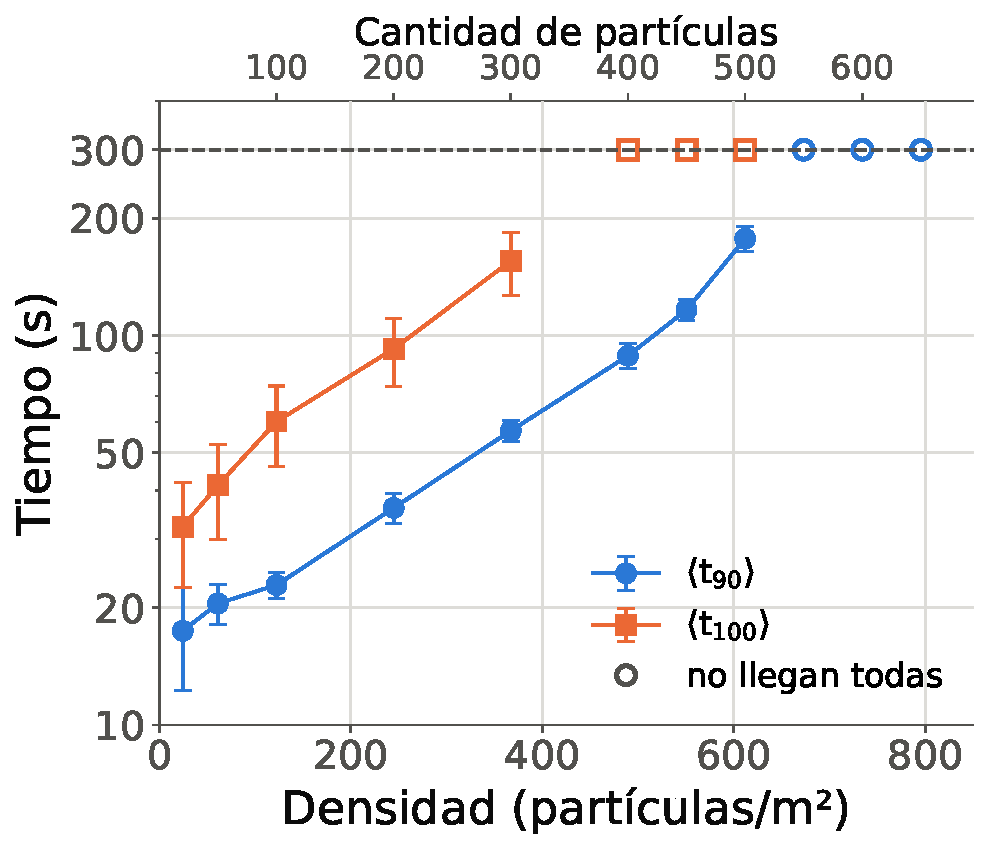
\includegraphics[width=\linewidth,height=5.3cm,keepaspectratio]{densidad-tiempos.pdf}
\end{column}
\begin{column}{.36\textwidth}
\ficha[accent]{Menor $\langle t_{90}\rangle$}{\densidadTexto}
\end{column}
\end{columns}
\end{frame}

\begin{frame}{Posición de los obstáculos}
\animacion{posicion}{%
  \ficha{Parámetros}{%
    $N=100$\par
    $\dt=\pasoElegido$ s}
  \ficha{Indicadores superiores}{%
    $\fu$ y $t_{90}$ de cada realización}
}{%
  \ficha{Velocidad $\times 2$}{%
    Reproducción al doble de la velocidad real.}}
\end{frame}

\begin{frame}{Posición: fracción de partículas usadas}
\figura{posicion-fu.pdf}{
\ficha{Configuración}{%
  $N=100$\par
  $t_f=100$ s}
\ficha{Estadística}{%
  Media $\pm$ desvío\par
  de 10 realizaciones}
}
\end{frame}

\begin{frame}{Posición: tiempo al 90\,\%}
\figura[.64]{posicion-t90.pdf}{
\ficha{Condiciones}{%
  $t_f=100$ s\par
  Media $\pm$ desvío de 10 realizaciones}
\ficha{Resultados}{\posicionTexto}
}
\end{frame}

\begin{frame}{Posición y densidad}
\figura[.68]{mapa-t90.pdf}{
\ficha{Condiciones}{%
  $t_f=100$ s\par
  Media de 10 realizaciones}
\ficha{Mínimos de conversión}{\mapaTexto}
}
\end{frame}

\begin{frame}{Distribución de rapideces}
\animacion{rapidez}{%
  \ficha{Configuración}{%
    $N=100$\par
    Sin obstáculos}
}{%
  \ficha{Cámara lenta}{%
    $1$ s simulado dura $2{,}5$ s.}}
\end{frame}

\begin{frame}{Rapidez: evolución de $f(v)$}
\figura{rapidez-evolucion.pdf}{
\ficha{Configuración}{%
  $N=100$\par
  Sin obstáculos}
\ficha{Estadística}{\rapidezRealizaciones{} realizaciones}
\ficha{Estacionario}{$t\geq\tEstacionario$ s}
}
\end{frame}

\begin{frame}{Rapidez: ajuste de Maxwell--Boltzmann}
\noindent{\small
  Estacionario: $t\geq\tEstacionario$ s\hfill
  \rapidezRealizaciones{} realizaciones\par}
\medskip
\begin{columns}[T,onlytextwidth]
\begin{column}{.49\textwidth}
\centering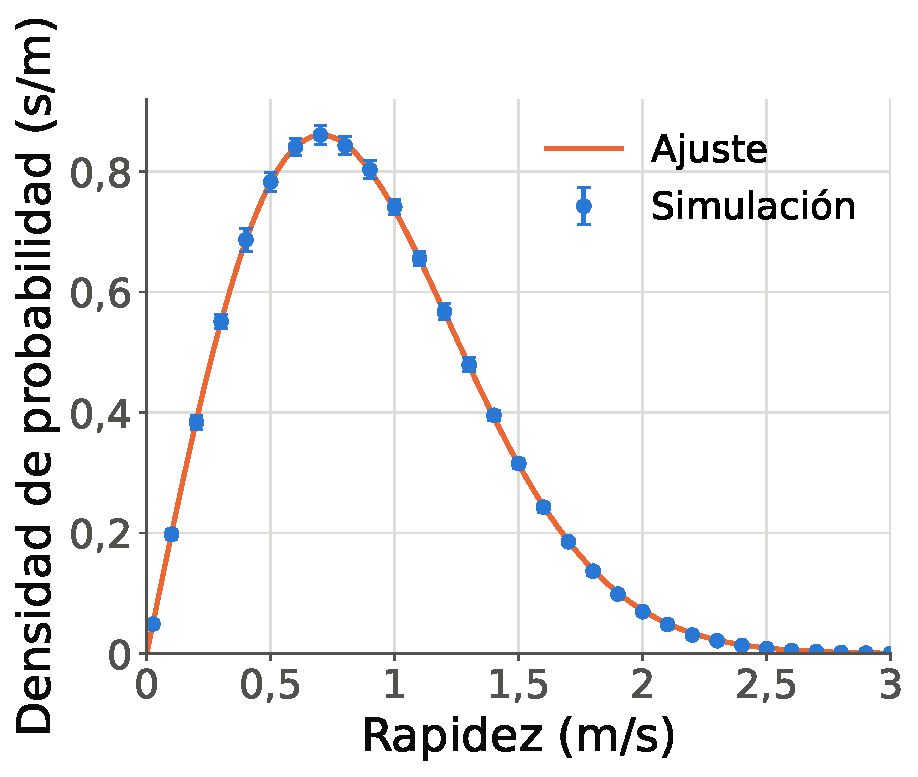
\includegraphics[width=\linewidth,height=3.7cm,keepaspectratio]{rapidez-ajuste.pdf}\par
\ficha{Distribución teórica}{%
  $\displaystyle f(v)=\frac{m v}{k_BT}\,e^{-m v^2/2k_BT}$}
\end{column}
\begin{column}{.49\textwidth}
\centering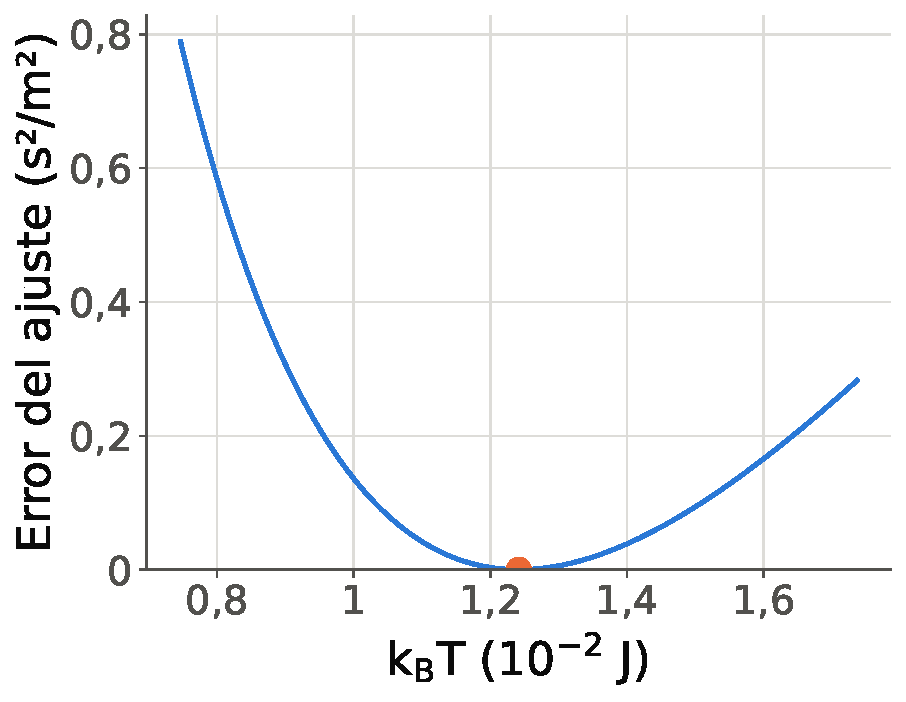
\includegraphics[width=\linewidth,height=3.7cm,keepaspectratio]{rapidez-error.pdf}\par
\ficha{Función de error}{%
  $\displaystyle E(k_BT)=\sum_i\big[f_i-f(v_i)\big]^2$\par\smallskip
  $v_i$: centro del bin $i$}
\end{column}
\end{columns}
\noindent{\small
  \textcolor{itbablue}{\textbf{Ajuste:}} $k_BT=\kbtAjuste$ J\hfill
  \textcolor{itbablue}{\textbf{Energía inicial:}} $m v_0^2/2=1{,}250\times10^{-2}$ J\par}
\end{frame}

\section{Conclusiones}
\begin{frame}\sectionpage\end{frame}

\begin{frame}{Conclusiones}
\begin{columns}[T,onlytextwidth]
\begin{column}{.48\textwidth}
\ficha{Integradores}{Beeman da el menor error, $\approx13\,\%$ menos que Verlet, con el mismo orden 2. Euler predictor-corrector es de orden 1.}
\ficha{Paso temporal}{$\delta E$ crece con $\dt$ y con el tiempo. $\dt=\pasoElegido$ s mantiene $\delta E<10^{-3}$ en $300$~s.}
\ficha{Costo}{El del TP4 crece en forma lineal con $N$ y el del TP3, mucho más rápido. El TP3 gana hasta $N=400$, pero con $N=650$ tarda 10 veces más.}
\end{column}
\begin{column}{.48\textwidth}
\ficha{Densidad}{Hay una densidad óptima: con $x_0=r$, $\langle t_{90}\rangle\approx20$ s es mínimo entre $N=20$ y 50. Con menos partículas faltan choques; con más, se estorban.}
\ficha{Posición}{Los extremos son los peores. Con $N$ de 50 a 200 el óptimo está en $x_0\approx0{,}16$--$0{,}26$ m. Con $N=20$, el mínimo es una meseta entre 0,11 y 0,40 m.}
\ficha{Rapidez}{En $\approx1$ s se llega a Maxwell--Boltzmann. El $k_BT$ ajustado difiere de $m v_0^2/2$ en un 0,7\,\%, del orden del desvío entre realizaciones.}
\end{column}
\end{columns}
\end{frame}

\begin{frame}{Declaración de uso de IA}
\begin{columns}[T,onlytextwidth]
\begin{column}{.46\textwidth}
\ficha{Herramientas utilizadas}{%
Codex con GPT-6.1 Sol.\\
Claude Code con Claude Opus 5.5.}
\end{column}
\begin{column}{.49\textwidth}
\ficha{Intervención}{%
Código C++ y Python, pruebas, ejecución de corridas y gráficos.}
\end{column}
\end{columns}
\end{frame}

\end{document}
